%%%%%%%%%%%%%%%%%%%%%%%%%%%%%%%%%%%%%%%%%%%%%%%%%%%%%%%%%%%%%%%%%%%%%%%%%%%%%%%%
% skip_list.tex
% An example demonstrating how to create a skip list in LaTeX with TikZ
% https://github.com/mhyee/latex-examples/
%%%%%%%%%%%%%%%%%%%%%%%%%%%%%%%%%%%%%%%%%%%%%%%%%%%%%%%%%%%%%%%%%%%%%%%%%%%%%%%%


% LaTeX Preamble
% Load packages and set options as needed
%%%%%%%%%%%%%%%%%%%%%%%%%%%%%%%%%%%%%%%%%%%%%%%%%%%%%%%%%%%%%%%%%%%%%%%%%%%%%%%%

% Set the document class to "article"
% Pass it "12pt" and "letterpaper" options
\documentclass[12pt,letterpaper]{article}

% We don't need the special font encodings, but still
% good practice to include these. See:
%
% http://tex.stackexchange.com/questions/664/why-should-i-use-usepackaget1fontenc
% http://dsanta.users.ch/resources/type1.html
\usepackage[T1]{fontenc}
\usepackage{ae,aecompl}
% http://tex.stackexchange.com/a/44699
% http://tex.stackexchange.com/a/44701
\usepackage[utf8]{inputenc}

% Use Latin Modern, an improved version of the Computer Modern font
\usepackage{lmodern}

% TikZ is what lets us draw graphics
\usepackage{tikz}
% chains lets us draw lines (or chains) between different nodes
\usetikzlibrary{chains}

% Disable page numbering
\pagestyle{empty}


% Define our own macros, for convenience
%%%%%%%%%%%%%%%%%%%%%%%%%%%%%%%%%%%%%%%%%%%%%%%%%%%%%%%%%%%%%%%%%%%%%%%%%%%%%%%%

% \ensuremath{ARG} is used to enable mathematics mode in a macro
% ARG will always be rendered in math mode,
% regardless of which mode the macro is called in
%
% http://www.giss.nasa.gov/tools/latex/ensuremath.html

% \snode{ID}{NUMBER} becomes \node{ID}[item]{\ensuremath{NUMBER}}
\newcommand{\snode}[2]{\node(#1)[item]{\ensuremath{#2}}}

% \nodelabel{SUBSCRIPT} becomes \node[label]{\ensuremath{S_SUBSCRIPT}}
\newcommand{\nodelabel}[1]{\node[label]{\ensuremath{S_#1}}}


% Begin the actual typesetting, by starting the "document" environment
%%%%%%%%%%%%%%%%%%%%%%%%%%%%%%%%%%%%%%%%%%%%%%%%%%%%%%%%%%%%%%%%%%%%%%%%%%%%%%%%
\begin{document}

% The final skip list will look something like this:
%
% S3 -infty                          +infty
% S2 -infty       6      24          +infty
% S1 -infty       6  16  24  31      +infty
% S0 -infty   5   6  16  24  31  39  +infty

% The nodes have the following IDs:
%       3a                           3h
%       2a       2d      2e          2h
%       1a       1c  1d  1e  1f      1h
%       0a   0b  0c  0d  0e  0f  0g  0h

% The IDs are used for "chaining" nodes together
% Note that S0, S1, S2, S3 are labels.
% Since they aren't chained, they don't need IDs

  \begin{center}
    % Draw the picture and set options
    % Enable chaining, and every node uses small font size
    % Note that "item" and "label" are types of nodes,
    % and have different styles specified
    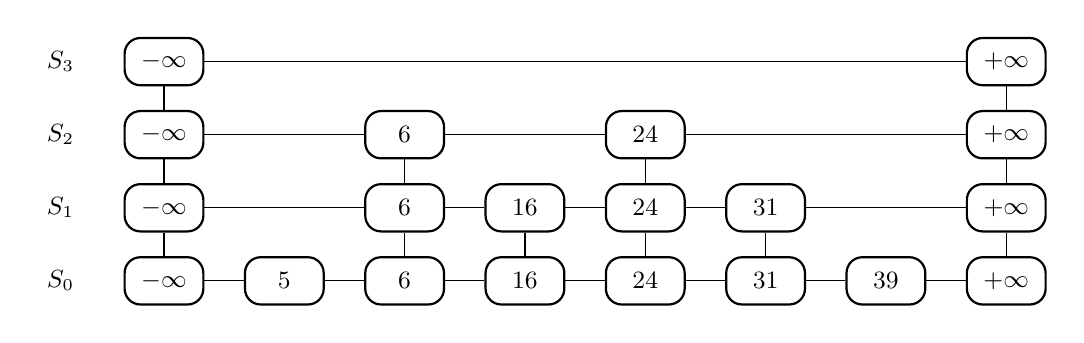
\begin{tikzpicture}[
        start chain,
        every node/.style={font=\small},
        item/.style={rectangle,minimum height=6mm,minimum width=10mm,
                     rounded corners=2mm,thick,draw=black},
        label/.style={rectangle,minimum size=6mm}
      ]

      % The nodes of the skip list are drawn in a matrix
      % \\ delimits the rows while & delimits the columns
      \matrix[row sep=3mm, column sep=5mm]{
        % Row 3: -infty ... +infty
        \nodelabel{3}; & \snode{3a}{-\infty}; & & & & & & & \snode{3h}{+\infty};\\

        % Row 2: -infty ... 6 ... 24 ... +infty
        \nodelabel{2}; & \snode{2a}{-\infty}; & & \snode{2c}{6}; & & \snode{2e}{24}; & & & \snode{2h}{+\infty};\\

        % Row 1: -infty ... 6 16 24 31 ... +infty
        \nodelabel{1}; & \snode{1a}{-\infty}; & & \snode{1c}{6}; & \snode{1d}{16}; & \snode{1e}{24}; & \snode{1f}{31}; & & \snode{1h}{+\infty};\\

        % Row 0: -infty 5 6 16 24 31 39 +infty
        \nodelabel{0}; & \snode{0a}{-\infty}; & \snode{0b}{5}; & \snode{0c}{6}; & \snode{0d}{16}; & \snode{0e}{24}; & \snode{0f}{31}; & \snode{0g}{39}; & \snode{0h}{+\infty};\\
      };

      % Start chaining the nodes together
      {
        % Horizontal chains
        % Specify a starting node (by ID), and join to other nodes (by going "through" them in an unbroken line)
        % Eg row 2: Start at 2a, join 2e, join 2h, join 2i
        [start chain] \chainin(0a); \chainin(0b) [join]; \chainin(0c) [join]; \chainin(0d) [join]; \chainin(0e) [join]; \chainin(0f) [join]; \chainin(0g) [join]; \chainin(0h) [join];
        [start chain] \chainin(1a); \chainin(1c) [join]; \chainin(1d) [join]; \chainin(1e) [join]; \chainin(1f) [join]; \chainin(1h) [join];
        [start chain] \chainin(2a); \chainin(2c) [join]; \chainin(2e) [join]; \chainin(2h) [join];
        [start chain] \chainin(3a); \chainin(3h) [join];
      }
      {
        % Vertical chains
        % Need to be separate chains from the horizontal ones
        [start chain] \chainin(0a); \chainin(1a) [join]; \chainin(2a) [join]; \chainin(3a) [join];
        [start chain] \chainin(0c); \chainin(1c) [join]; \chainin(2c) [join];
        [start chain] \chainin(0d); \chainin(1d) [join];
        [start chain] \chainin(0e); \chainin(1e) [join]; \chainin(2e) [join];
        [start chain] \chainin(0f); \chainin(1f) [join];
        [start chain] \chainin(0h); \chainin(1h) [join]; \chainin(2h) [join]; \chainin(3h) [join];
      }
    \end{tikzpicture}
  \end{center}

\end{document}
